\documentclass{article}
\usepackage[text={6in,9in}]{geometry}
\usepackage{graphicx}
\usepackage{hyperref}
\usepackage[europeanresistors,europeaninductors]{circuitikz}

\title{Naive Circuit Simulation in Pure Haskell}
\author{Johannes Waldmann, HTWK Leipzig}
\begin{document}
\maketitle

\section{Motivation}

For my lecture on Computer Music, 
I wanted to show  the behaviour
of electrical oscillators and filters.

The plan was to ``solve'' the differential equation
that describes the system by simulation, that is,
by treating it as a difference equation.

The goal is not to make an exact simulation of circuits.
There are tools for that (SPICE, Matlab)
but their source code is not available for inspection.

The goal is to make a simulation of idealized circuits
where students can read and understand the source.

A technical goal is to use Haskell as an implementation language,
and no non-Haskell (e.g., numerical) libraries.
This allows to build exercises on circuits as part
of my \texttt{autotool} e-learning system.

\section{Example}

The circuit shown on the left
is represented by the textual description shown on the right

\begin{minipage}[b]{0.5\linewidth}
   \begin{circuitikz}[scale=0.8]
    \draw (0,3) node [left]{$U_E$}
    to [short,i=$I$,*-] (1,3)
    to [R,l=$R$, -*] (4,3)
    to [L,l=$L$] (4,1) node [ground] {}
    (4,3) to [short,-*] (6,3)
    to [C,l=$C$] (6,1) node [ground] {}
    (6,3) to [short,-*] (8,3) node [right] {$U_A$} ;
  \end{circuitikz},
\end{minipage}
\begin{minipage}[b]{0.5\linewidth}
\begin{verbatim}
bp = Circuit
  { ground = 0, output = 2
  , components = fromList
    [ (1, Voltage_Source_Input, 0)
    , (1, Resistor  (Ohm   1), 2)
    , (2, Capacitor (Farad 1), 0)
    , (2, Inductor (Henry 1), 0)
    ]
  }
\end{verbatim}
\end{minipage}


The following command runs a simulation with 1000 steps of 0.02 seconds each,
where the input is an impulse, and renders the output function to a file
(it could also render to an X11 window)

\begin{minipage}[b]{0.5\linewidth}
\begin{verbatim}
main = plotList [ EPS "data/BP.eps" ] 
     $ take 1000 
     $  apply_func bp (Second 0.02) 
     $ impulse (Second 0.1) (Volt 1)



\end{verbatim}
  \end{minipage}
\begin{minipage}[b]{0.5\linewidth}
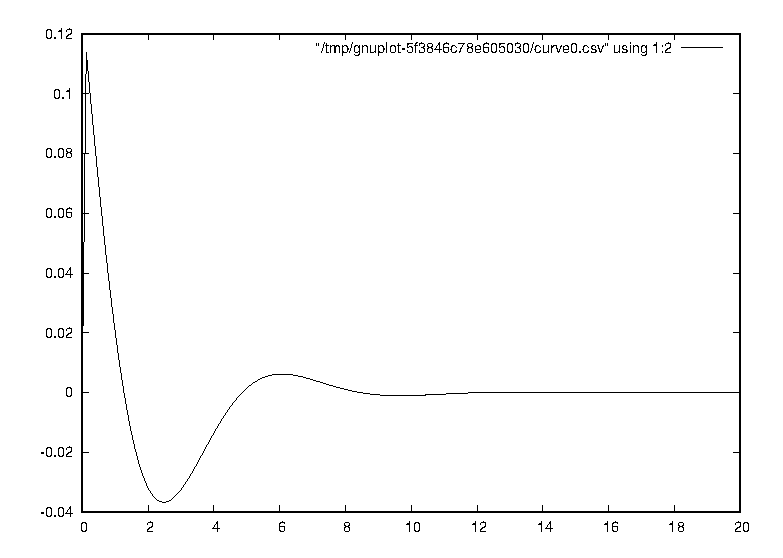
\includegraphics[height=5cm]{BP}
\end{minipage}

Complete source code is at
\url{https://gitlab.imn.htwk-leipzig.de/waldmann/circuit}.
The initial working version (producing the above output) 
contains 1626 lines of source code.

\section{Data}

A circuit has a designated ground node, an output node,
and contains components. Each component is situated on an edge between two nodes.
\begin{verbatim}
data Circuit = Circuit
  { ground :: Node
  , output :: Node
  , components :: M.Map Edge (Node, Component, Node)
  } deriving Show
\end{verbatim}

Circuits may use these components:
\begin{verbatim}
data Component
  = Resistor Resistance
  | Capacitor Capacitance
  | Inductor Inductance
  | Current_Source Current
  | Voltage_Source Voltage
  | Voltage_Source_Input
  | Opamp { pos :: Node, neg :: Node }
\end{verbatim}

\section{Operation}

The \emph{state} of a circuit (at some step during the simulation)
is a mapping from capacitors to voltage,
and from inductors to current.

A step of the simulation computes the next state as follows:
\begin{itemize}
\item replace  \verb|Voltage_Source_Input| with voltage source containing current input value,
  $C$ with voltage source, $L$ with current source, according to previous state,
\item build and solve Kirchhoff's equations for voltages at nodes ($U_p$), currents through edges ($I_e$)
  \begin{itemize}
  \item For each node, sum of currents is zero. 
  \item For each edge $e$ from $p$ to $q$, with $U_e=U_p-U_q$: if its component is
    \begin{itemize}
    \item resistor $R$: Ohm's law $U_e = R\cdot I_e$
    \item voltage source $U_S$: $U_e=U_S$
    \item current source $I_S$: $I_e = I_S$
    \item opamp with positive input node $n_+$, negative input node $n_-$,:
      $U_e=G\cdot(U_{n_+}-U_{n_-})$, where $G$ is the (fixed) gain of the amplifier.
    \end{itemize}
  \end{itemize}
\item from the solution, compute differentials for state components
(capacitor: $I = C dU/dt$, inductor $U = L dI/dt$), and update (proportional to time slice of simulation)
\end{itemize}

We model input voltage as \verb|Voltage_Source|,
so we don't need a special case here (the solver will compute the input current).
Same for output nodes of opamps (solver will compute current).



\end{document}
